\documentclass[8pt, a4paper, onesided]{article}
\usepackage[left=0.1in,right=0.1in,top=0.1in,bottom=0.1in,headsep=0.05in]{geometry}
\usepackage{hyperref}
\usepackage{fancyhdr}
\usepackage{listings}
\usepackage{xcolor}
\usepackage{tocloft}
\usepackage{pdflscape}
\usepackage{multicol}
\usepackage{titlesec}
\usepackage{minted}
\usepackage{amsmath}
\usepackage{graphicx}

\usemintedstyle{default}

\setlength{\columnsep}{0.4cm}
\setlength{\columnseprule}{0.1pt}
\setlength{\parskip}{-4.5mm plus 0.5mm minus 0.5mm}

\setlength{\fboxsep}{1pt}%
\setlength{\fboxrule}{0.01pt}%

\titleformat{\section}{\normalfont\fontsize{12}{15}\bfseries}{\thesection}{1em}{}
\titleformat{\subsection}{\normalfont\fontsize{10}{13}\bfseries}{\thesubsection}{0.5em}{}
%\titleformat{\subsection}{\normalfont\bfseries}{\thesubsection}{1em}{}[\vspace*{-3.75ex}]
%\titlespacing*{\subsection}
%{0pt}{-1.75ex plus 1ex minus 1ex}{-2ex plus 1ex minus 1ex}

%\renewcommand{\ttdefault}{pcr}
\renewcommand\cftsecfont{\fontsize{10}{11}\bfseries}
\renewcommand\cftsecpagefont{\fontsize{10}{11}\mdseries}
\renewcommand\cftsubsecfont{\fontsize{8}{9}\mdseries}
\renewcommand\cftsubsecpagefont{\fontsize{8}{9}\mdseries}
\renewcommand\cftsecafterpnum{\vspace{-0.5ex}}
\renewcommand\cftsubsecafterpnum{\vspace{-0.5ex}}

\renewcommand{\theFancyVerbLine}{
  \sffamily\textcolor[rgb]{1.5,0.5,0.5}{\scriptsize\arabic{FancyVerbLine}}}
  
\lstset{escapechar=\$}

\setminted{breaklines, breaksymbolleft=\space,
breakafter={,+-*;>=}, breakbefore={</}, tabsize=2, obeytabs, mathescape, frame=topline, fontsize=\fontsize{10}{12}}

\renewcommand{\headrulewidth}{0pt}
\pagestyle{fancy}
\fancyhead[L]{}
\fancyhead[R]{}
\fancyfoot[C]{}

\fancypagestyle{plain}
{
\fancyhead[L]{}
\fancyhead[R]{}
\fancyfoot[C]{}
}

\title{\vspace{-2.5ex}\Large{KUET\_ThunderBolt Team Notebook\\\today}}
\author{Muhiminul Islam Osim, Toufiq Imam Nuhash,\\Sharif Minhazul Islam}
\date{}

\graphicspath{ {./images} }

\begin{document}
%\begin{landscape}
\begin{multicols*}{2}

\maketitle
\vspace{-7ex}
\tableofcontents
\pagestyle{fancy}
 
\raggedbottom
\input contents.tex
\end{multicols*}
%
%\begin{figure}[]
%    \centering
%    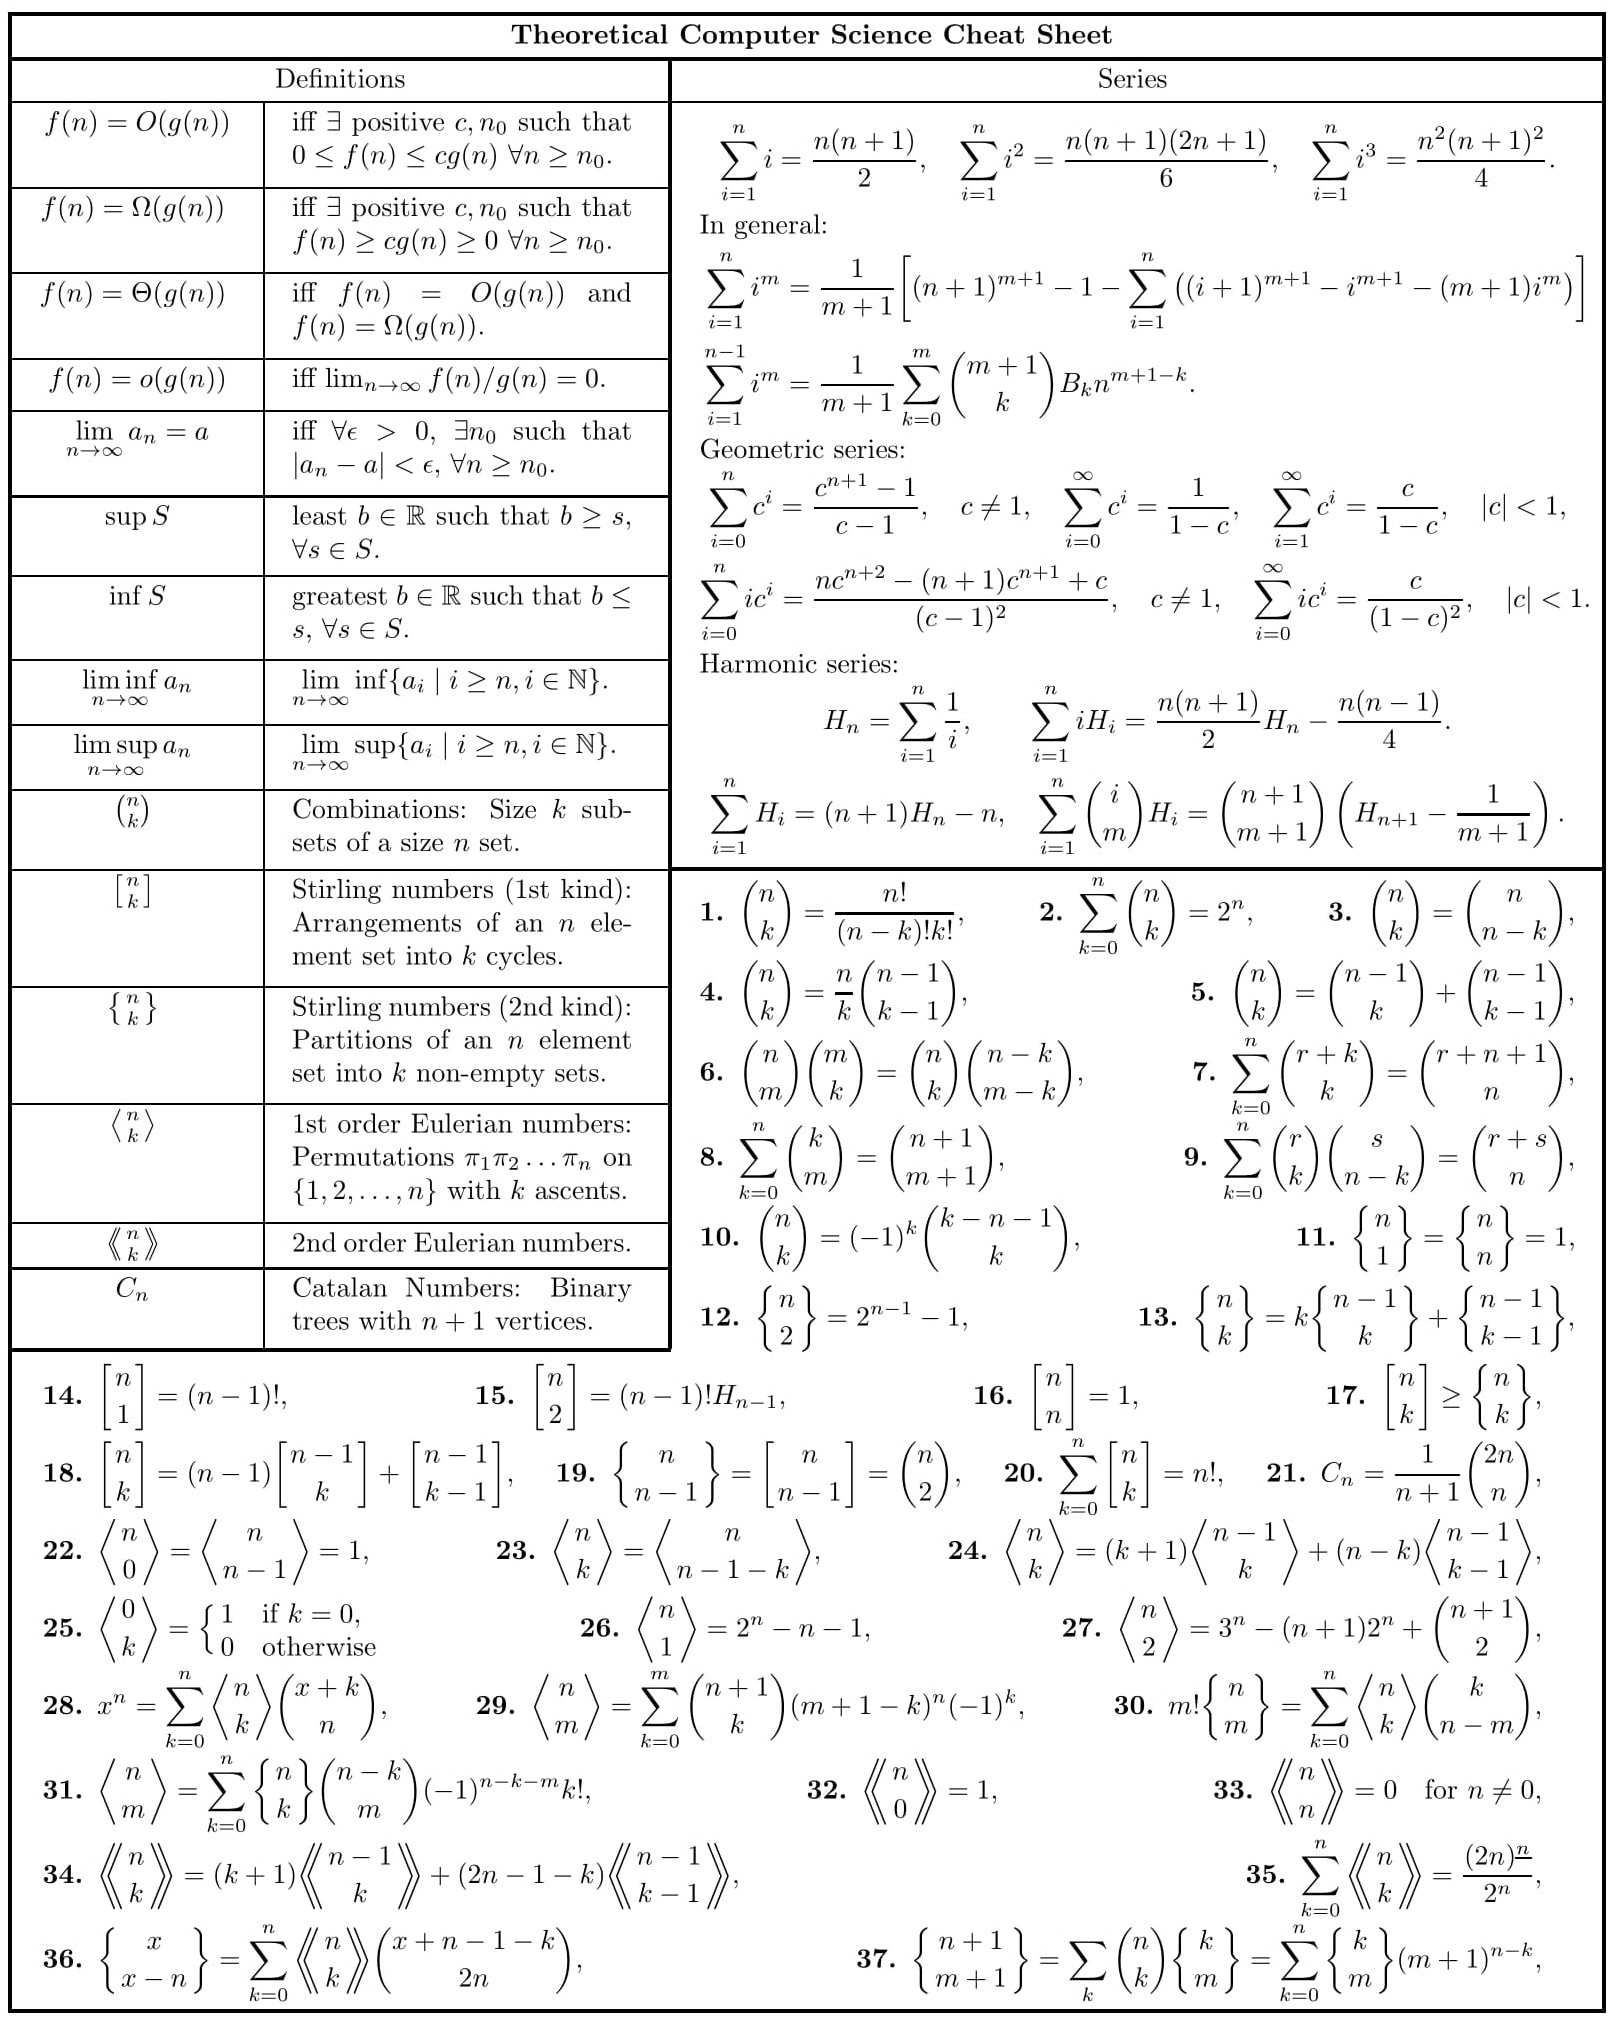
\includegraphics[width=\textheight/3, angle=90]{form0}\\
%    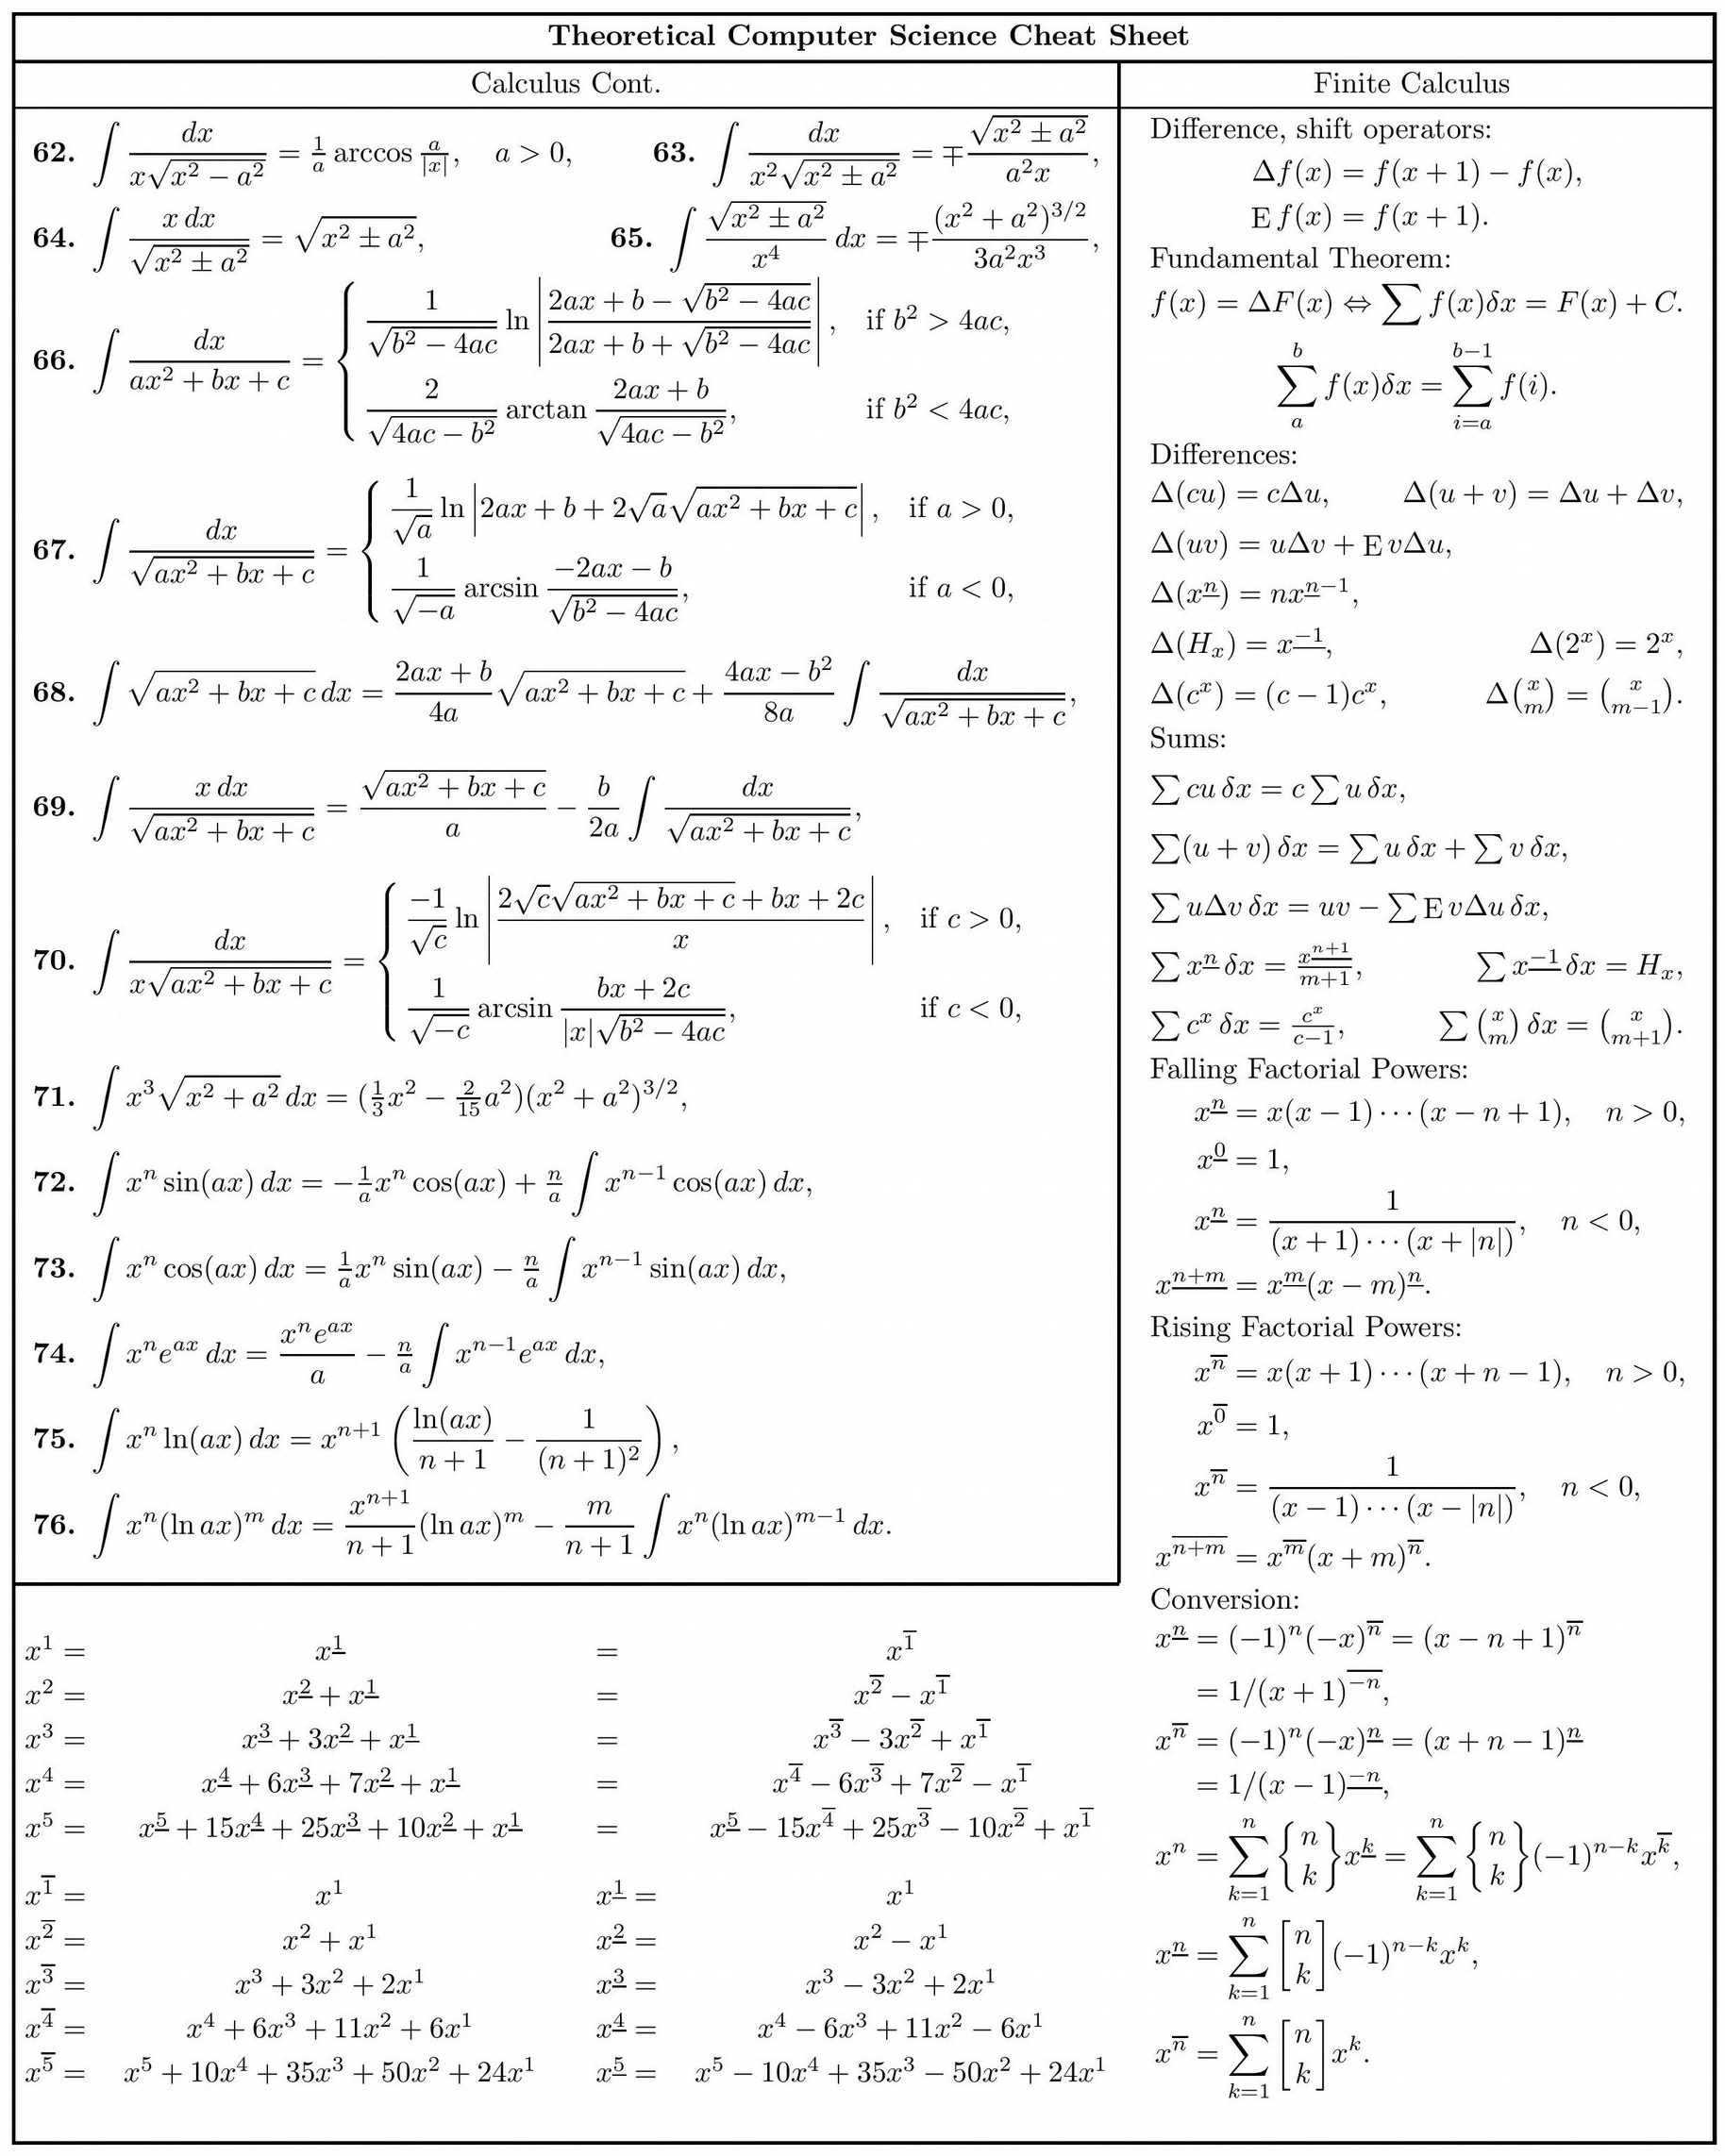
\includegraphics[width=\textheight/3, height=\textwidth - 4.25cm, angle=90]{form1}\\
%    \fbox{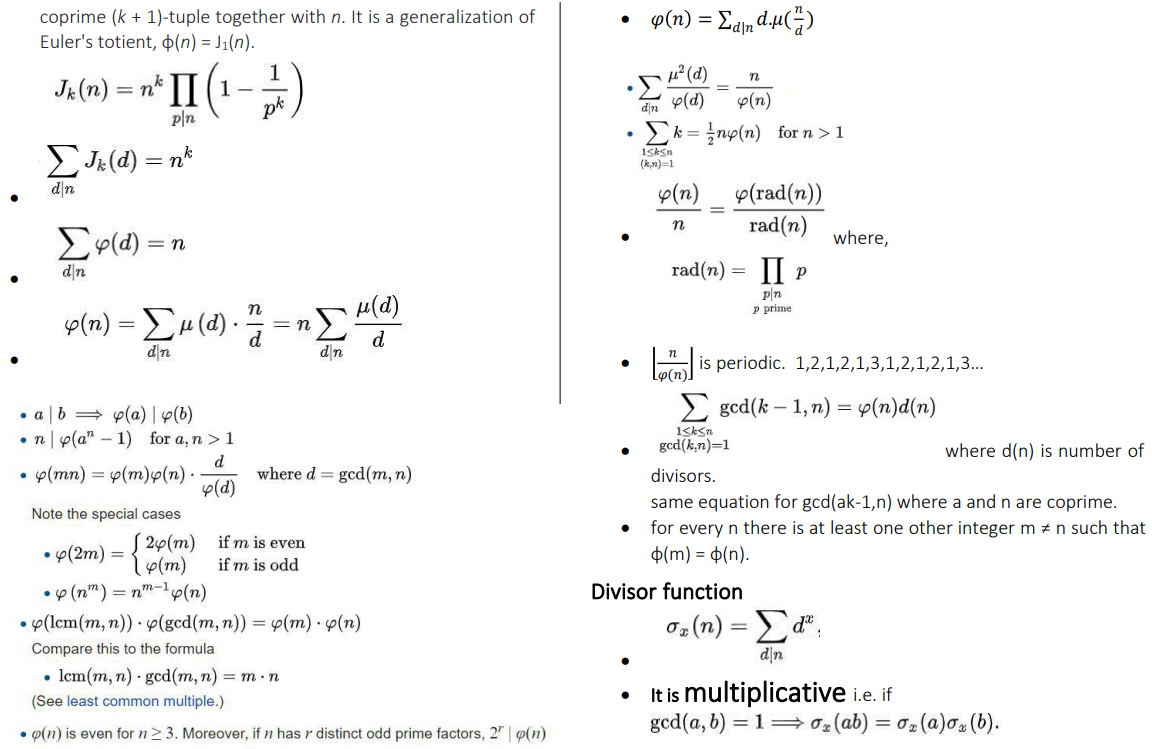
\includegraphics[height=\textheight/3, angle=0]{1}}
%\end{figure}
%\begin{figure}[]
%    \centering
%    \fbox{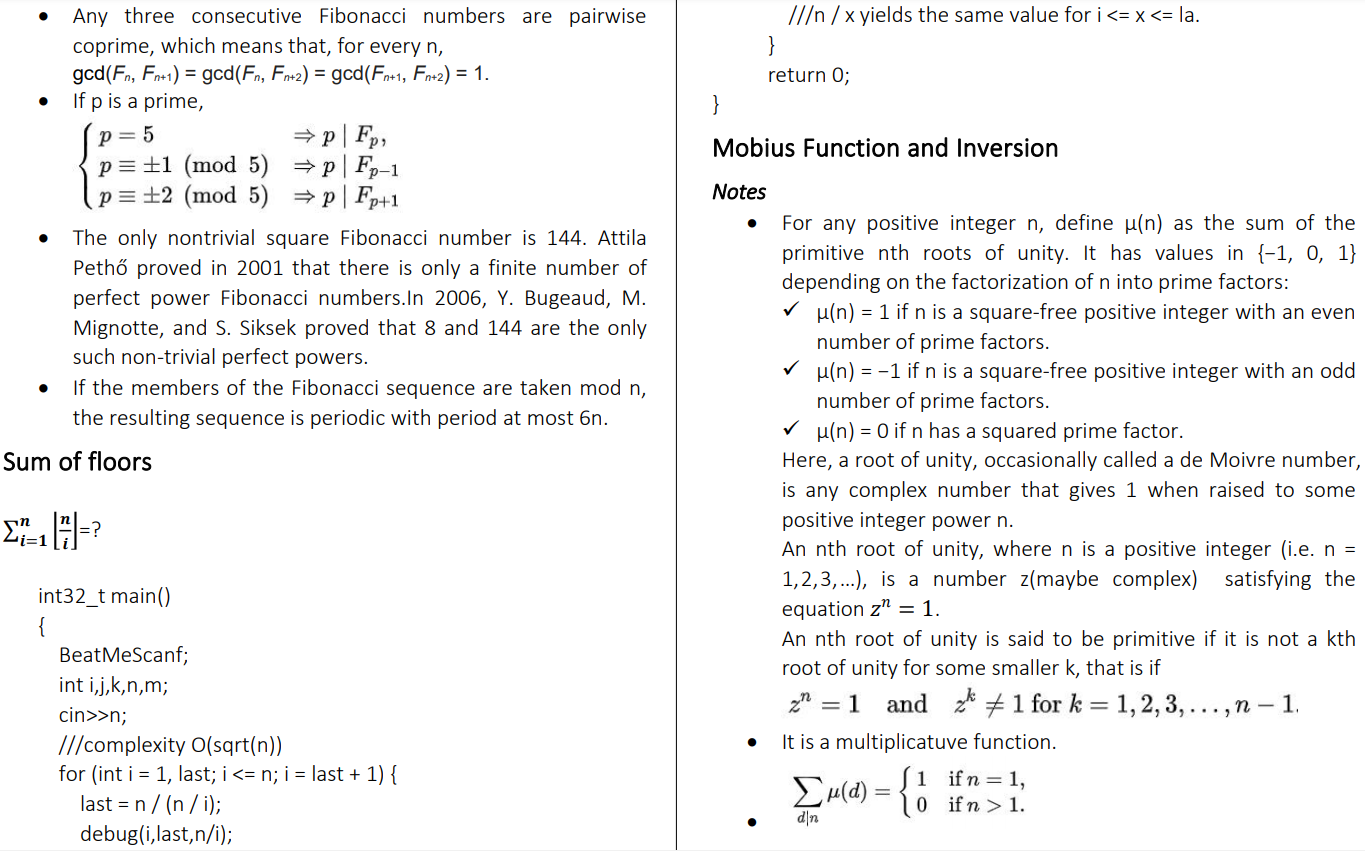
\includegraphics[height=\textheight/3, angle=0]{2}}\\
%    \fbox{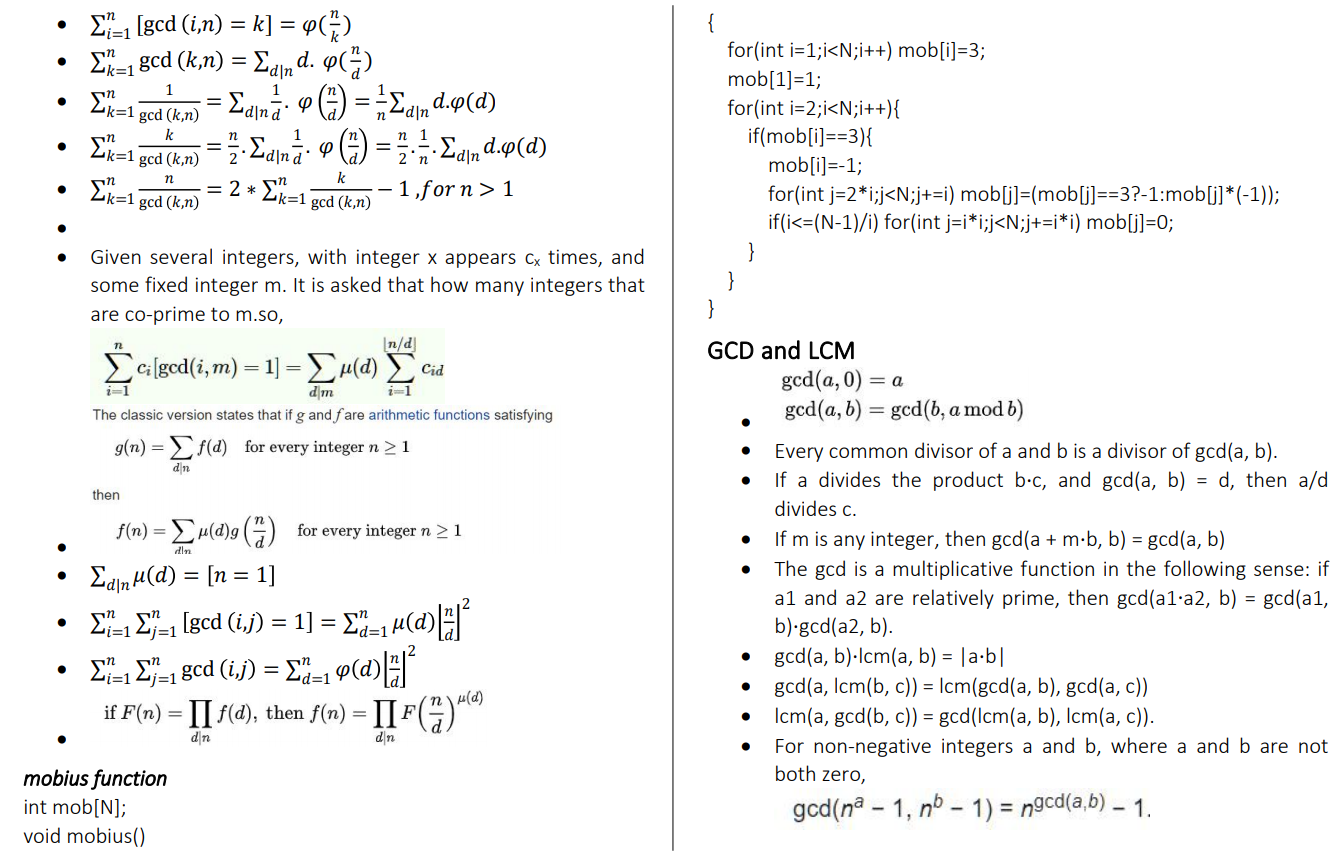
\includegraphics[height=\textheight/3, angle=0]{3}}\\
%    \fbox{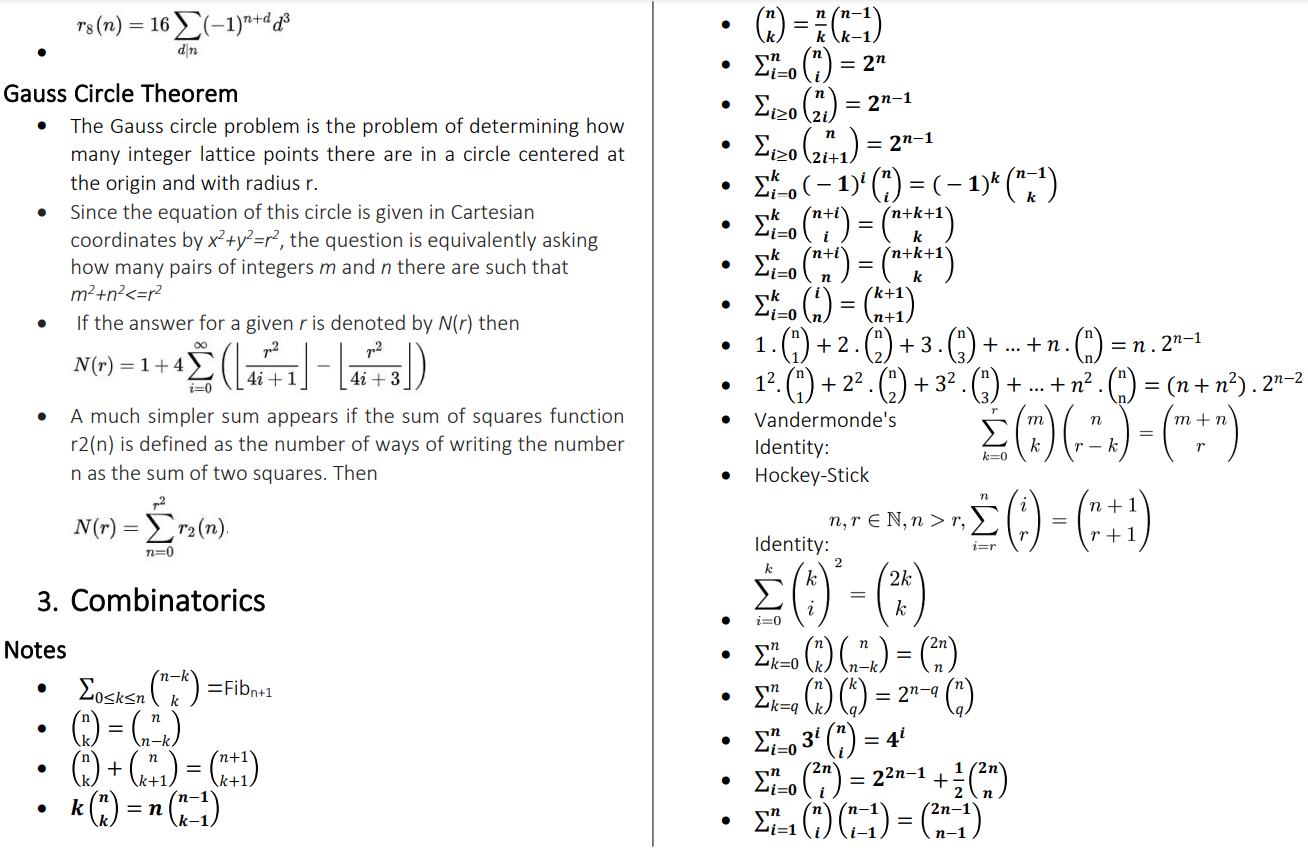
\includegraphics[height=\textheight/3, angle=0]{4}}
%\end{figure}
%\begin{figure}[]
%    \centering
%    \fbox{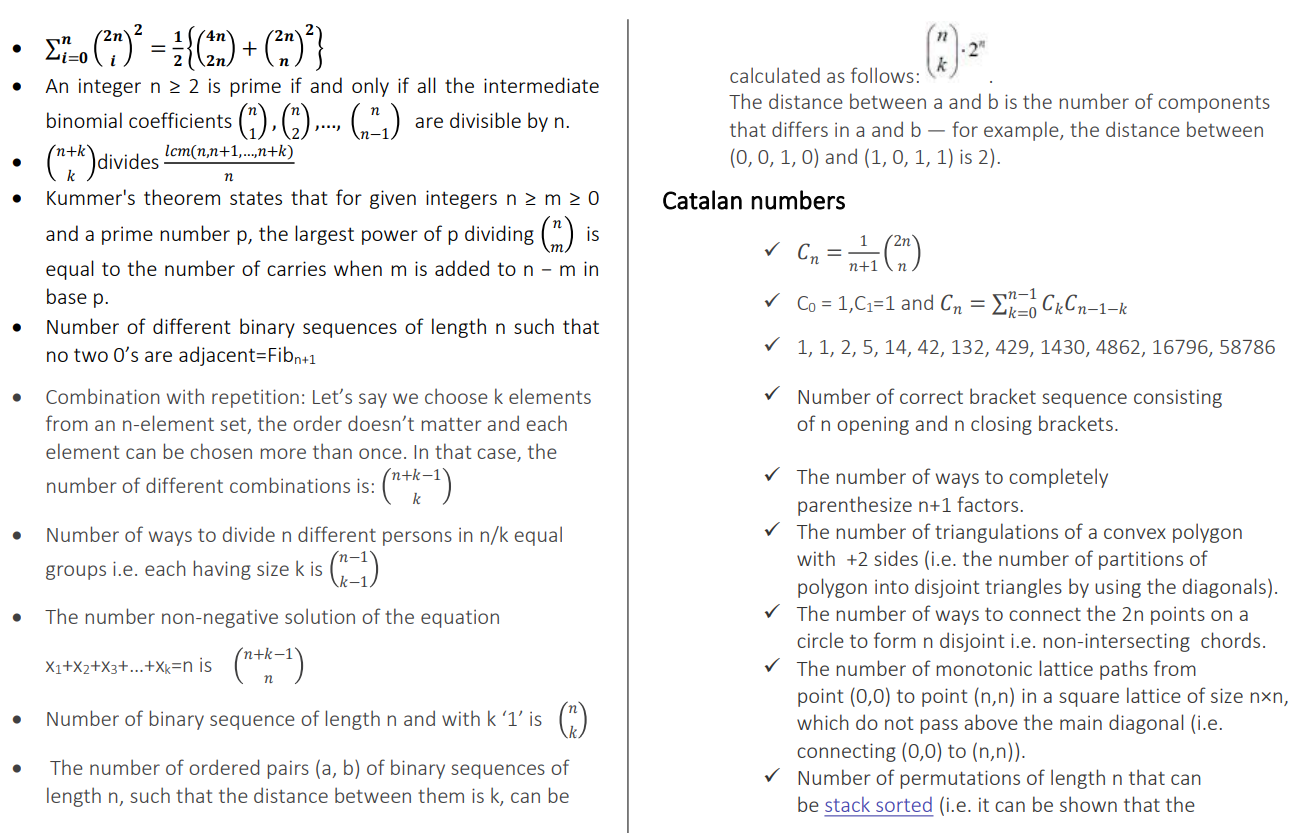
\includegraphics[height=\textheight/3, angle=0]{5}}\\
%    \fbox{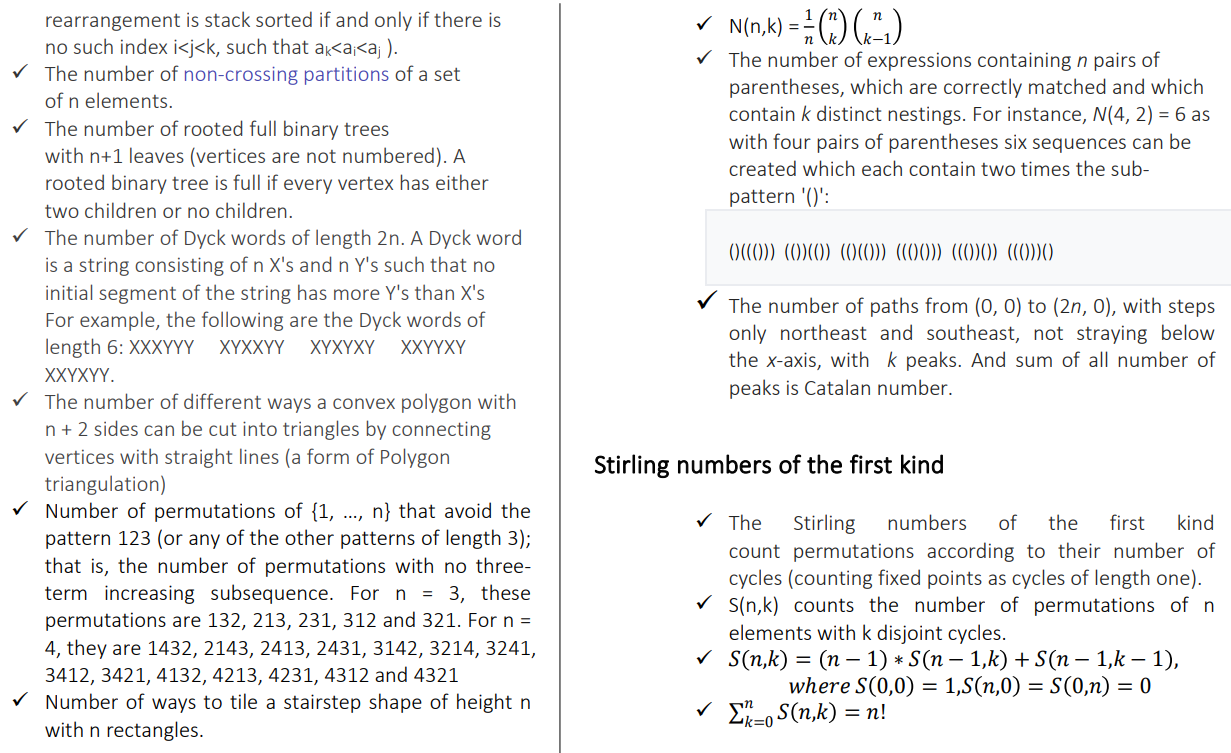
\includegraphics[height=\textheight/3, angle=0]{6}}\\
%    \fbox{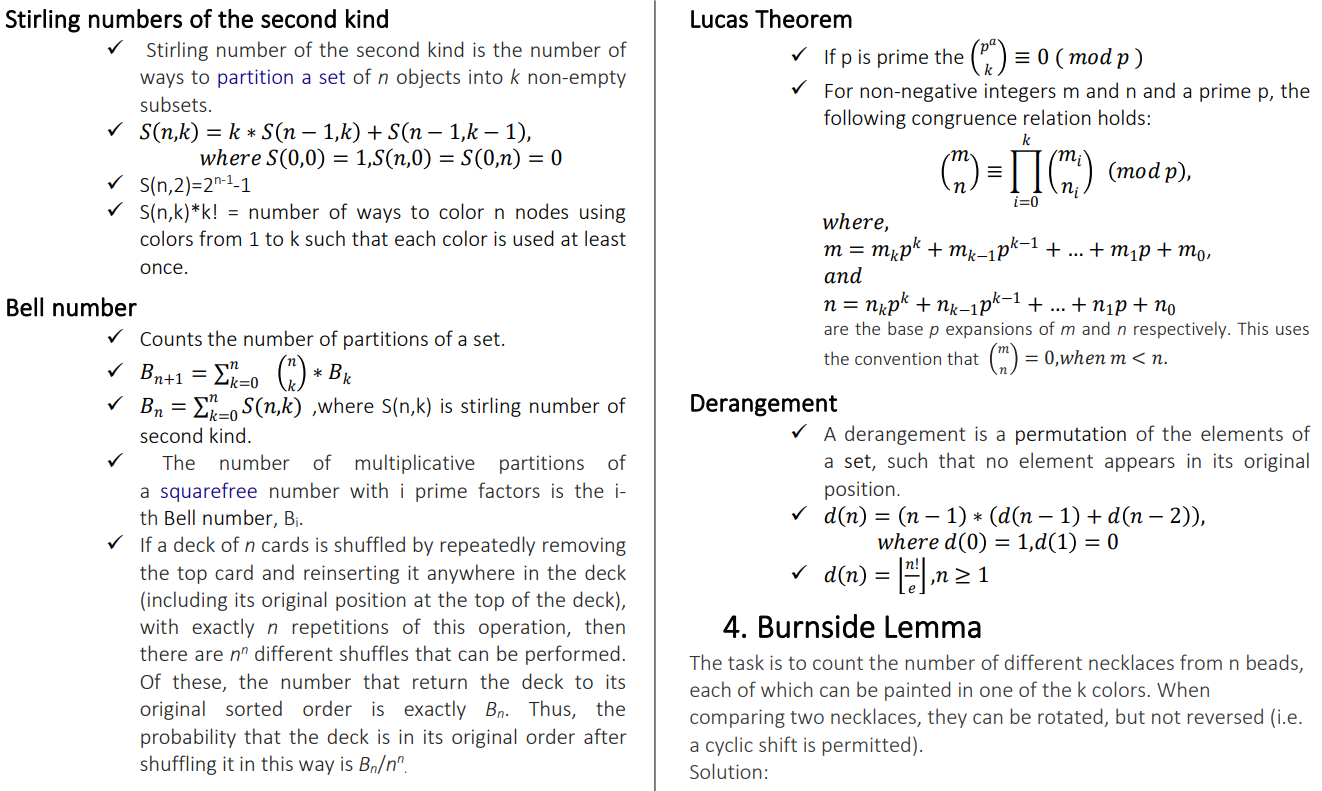
\includegraphics[height=\textheight/3, angle=0]{7}}
%\end{figure}

%\end{landscape}
\end{document}
